\documentclass[border=10pt]{standalone}
\usepackage{pgfplots}
\pgfplotsset{compat=1.18}
\begin{document}
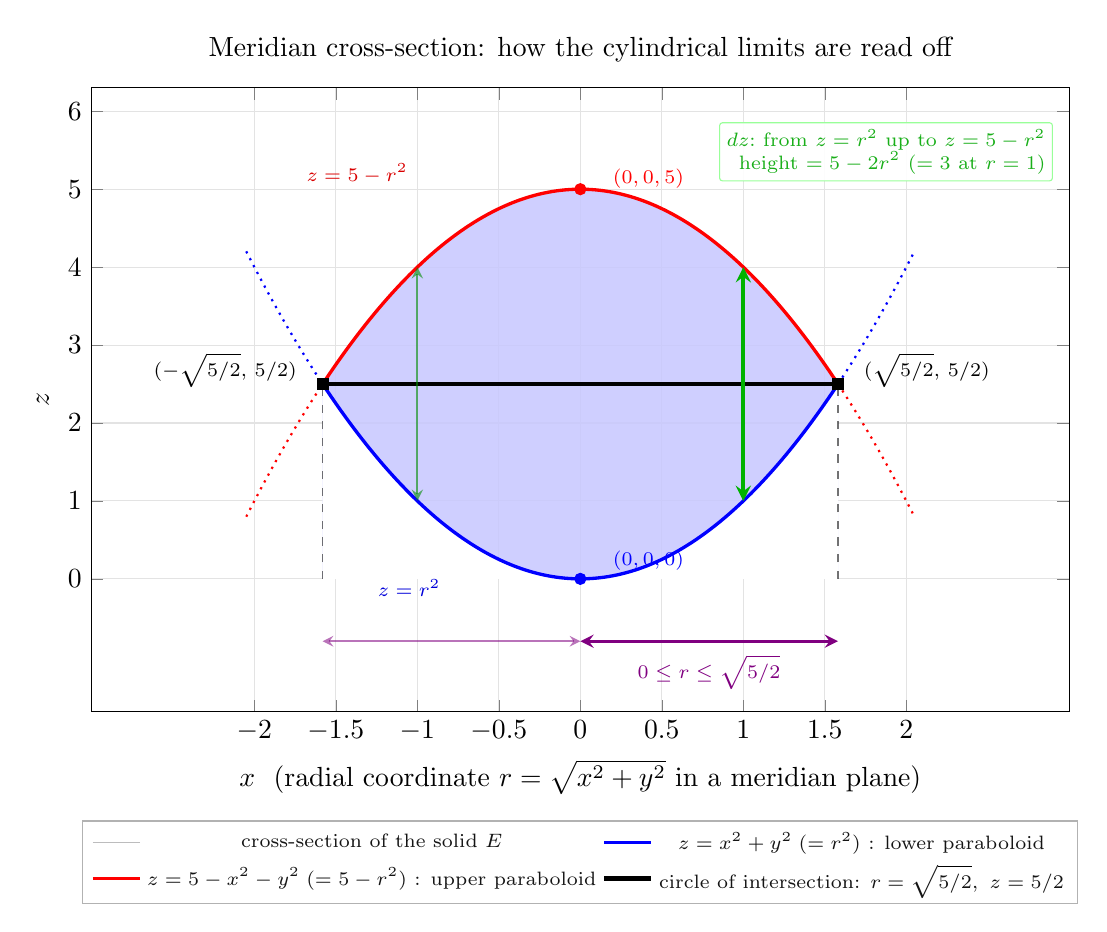
\begin{tikzpicture}
\begin{axis}[
    width=14cm, height=9.5cm,
    xmin=-3.0, xmax=3.0, ymin=-1.7, ymax=6.3,
    xtick={-2,-1.5,...,2}, ytick={0,1,...,6},
    xlabel={$x$\ \ (radial coordinate $r=\sqrt{x^2+y^2}$ in a meridian plane)},
    ylabel={$z$},
    grid=major, grid style={gray!22},
    axis x line=box, axis y line=box,
    legend style={at={(0.5,-0.175)}, anchor=north, font=\scriptsize,
                  draw=black!30, fill=white, fill opacity=0.92, legend columns=2},
    title={Meridian cross-section: how the cylindrical limits are read off},
]
% ---- filled region = cross-section of the solid (upper curve, then white cut-out) ----
\addplot[fill=blue!22, opacity=0.85, draw=none, domain=-1.5811:1.5811, samples=120]
  {5-x^2} \closedcycle;
\addlegendentry{cross-section of the solid $E$}
\addplot[fill=white, draw=none, forget plot, domain=-1.5811:1.5811, samples=120]
  {x^2} \closedcycle;
% ---- lower / upper paraboloid over the disk ----
\addplot[blue, very thick, domain=-1.5811:1.5811, samples=120] {x^2};
\addlegendentry{$z=x^2+y^2\;(=r^2)$ : lower paraboloid}
\addplot[red, very thick, domain=-1.5811:1.5811, samples=120] {5-x^2};
\addlegendentry{$z=5-x^2-y^2\;(=5-r^2)$ : upper paraboloid}
% ---- parts of the paraboloids outside the solid (dotted) ----
\addplot[blue, dotted, thick, forget plot, domain=1.5811:2.05, samples=40] {x^2};
\addplot[blue, dotted, thick, forget plot, domain=-2.05:-1.5811, samples=40] {x^2};
\addplot[red, dotted, thick, forget plot, domain=1.5811:2.05, samples=40] {5-x^2};
\addplot[red, dotted, thick, forget plot, domain=-2.05:-1.5811, samples=40] {5-x^2};
% ---- horizontal chord = intersection circle seen edge-on ----
\addplot[black, ultra thick] coordinates {(-1.5811,2.5) (1.5811,2.5)};
\addlegendentry{circle of intersection: $r=\sqrt{5/2},\ z=5/2$}
% ---- dashed projections to the x-axis ----
\addplot[black, dashed, thin, opacity=0.55, forget plot] coordinates {(-1.5811,0) (-1.5811,2.5)};
\addplot[black, dashed, thin, opacity=0.55, forget plot] coordinates {(1.5811,0) (1.5811,2.5)};
% ---- the dz element at r = 1 (plus its mirror at r = -1) ----
\addplot[green!70!black, line width=1.4pt, <->, >=stealth, forget plot] coordinates {(1,1) (1,4)};
\addplot[green!55!black, line width=0.8pt, <->, >=stealth, opacity=0.6, forget plot] coordinates {(-1,1) (-1,4)};
% ---- r-range arrows ----
\addplot[violet, line width=1.1pt, <->, >=stealth, forget plot] coordinates {(0,-0.8) (1.5811,-0.8)};
\addplot[violet, line width=0.7pt, <->, >=stealth, opacity=0.55, forget plot] coordinates {(-1.5811,-0.8) (0,-0.8)};
% ---- key points ----
\addplot[only marks, mark=*, red, forget plot] coordinates {(0,5)};
\addplot[only marks, mark=*, blue, forget plot] coordinates {(0,0)};
\addplot[only marks, mark=square*, black, forget plot] coordinates {(-1.5811,2.5) (1.5811,2.5)};
% ---- text annotations ----
\node[red,  font=\scriptsize] at (axis cs:0.14,5.14) [anchor=west] {$(0,0,5)$};
\node[blue, font=\scriptsize] at (axis cs:0.14,0.24) [anchor=west] {$(0,0,0)$};
\node[font=\scriptsize] at (axis cs:1.68,2.68) [anchor=west] {$(\sqrt{5/2},\,5/2)$};
\node[font=\scriptsize] at (axis cs:-1.68,2.68)[anchor=east] {$(-\sqrt{5/2},\,5/2)$};
\node[green!65!black, font=\scriptsize, align=right, anchor=south east,
      fill=white, fill opacity=0.9, inner sep=2.5pt, rounded corners=1pt, draw=green!40]
      at (axis cs:2.9,5.1)
      {$dz$:\ from $z=r^2$ up to $z=5-r^2$\\ height $=5-2r^2$ ($=3$ at $r=1$)};
\node[violet, font=\scriptsize] at (axis cs:0.79,-0.85) [anchor=north] {$0\le r\le\sqrt{5/2}$};
\node[blue!85!black, font=\scriptsize, anchor=north]  at (axis cs:-1.05,0.12) {$z=r^2$};
\node[red!85!black,  font=\scriptsize, anchor=south east] at (axis cs:-1.0,4.95) {$z=5-r^2$};
\end{axis}
\end{tikzpicture}
\end{document}
